\documentclass[runningheads,a4paper]{llncs}
\usepackage[T1]{fontenc}
\usepackage[utf8]{inputenc}
\usepackage{graphicx,booktabs,amsmath,amssymb,array,microtype,url}
\usepackage[hidelinks]{hyperref}
\setlength{\emergencystretch}{2em}
\graphicspath{{figures/}}
\renewcommand\UrlFont{\rmfamily}
\newcommand{\HergDelta}{0.094}
\newcommand{\HergCI}{[0.051, 0.145]}
\newcommand{\DiliDelta}{0.020}
\newcommand{\DiliCI}{[-0.009, 0.051]}
\newcommand{\AmesDelta}{0.005}
\newcommand{\AmesCI}{[-0.007, 0.016]}
\newcommand{\HergP}{0.009}
\newcommand{\HergScratchP}{0.009}
\newcommand{\HergDropP}{0.005}
\newcommand{\DiliScratchQ}{0.034}
\newcommand{\DiliScratchP}{0.137}
\newcommand{\HfHergSeed}{0.872}
\newcommand{\HfHergEnsemble}{0.874}
\newcommand{\HfRandomSeed}{0.771}
\newcommand{\HfRandomEnsemble}{0.838}
\newcommand{\HergTunedPre}{0.916}
\newcommand{\HergTunedRandom}{0.790}
\newcommand{\HergSplitMin}{0.039}
\newcommand{\HergSplitMax}{0.138}
\newcommand{\LowDeltas}{0.026, 0.089, 0.097, 0.122}
\newcommand{\LowFiftyCI}{[-0.134, 0.220]}
\newcommand{\MaxProbDrift}{0.065716}
\newcommand{\TestDriftMin}{-0.046919}
\newcommand{\TestDriftMax}{0.145370}
\newcommand{\FpHergGaps}{0.123/0.132/0.127}
\newcommand{\BfHergGaps}{0.122/0.120/0.087}
\newcommand{\PoolIndependent}{0.902905}
\newcommand{\ShiftIndependent}{0.873281}
\newcommand{\PoolReused}{0.897033}
\newcommand{\ShiftReused}{0.866167}

\begin{document}
\title{Auditing ADMET Foundation-Model Claims:\\Capacity Controls, Corpus Exposure, and Calibration Shift}
\titlerunning{Auditing ADMET Foundation-Model Claims}
\author{Anonymous authors}
\authorrunning{Anonymous authors}
\institute{Research manuscript: exploratory evaluation under inherited source labels}
\maketitle
\begin{abstract}
Molecular foundation-model comparisons can conflate pretrained weights with architecture, data identity, numerical execution, and calibration design. We audit a CheMeleon case study on hERG, DILI, and Ames using source-file reconstruction, computation-matched controls, five global structure-grouped partitions, and separated selection and calibration sets. Across 25 fits per model and endpoint, the mean AUROC advantage over a same-capacity random encoder is \HergDelta{} for hERG (conditional 95\% interval \HergCI{}), \DiliDelta{} for DILI (\DiliCI{}), and \AmesDelta{} for Ames (\AmesCI{}). The latter intervals include zero and do not establish equivalence. Historical controls used different aggregation operators. Repeated BF16 inference also proved unstable; all new neural outcomes therefore use separately stored deterministic FP32 predictions, verified by full fixed-weight replay. Reconstructing 944,296 released corpus records establishes file-level structural matching, not label leakage or a causal exposure benefit. An equal-size, randomized held-out-pool diagnostic separates calibration reuse from an observational domain contrast. The resulting audit supports endpoint-specific conclusions and an explicit claim-to-artifact chain. Assay-level provenance remains incomplete; the results are exploratory rather than approved external validation.
\keywords{Molecular machine learning \and Reproducibility \and Evaluation fairness \and Conformal prediction \and ADMET}
\end{abstract}

\section{Introduction}
Absorption, distribution, metabolism, excretion, and toxicity (ADMET) predictions influence costly compound-selection decisions. Improvements over small random networks need not identify pretraining benefits: capacity, pooling, optimization, molecular identity dependencies, and numerical execution can change the comparison. Likewise, observations used for predictor selection need not supply independent calibration.

We audit a CheMeleon-based repository and its source snapshots, rather than replicate every official result. Architecture/fine-tuning ablations and broad repeated-split ADMET benchmarks already exist~\cite{burns2025chemeleon,zhao2026revisiting}. We instead reconstruct the evidence chain and re-evaluate specific implementation failures.

We ask whether an advantage persists with the same computation, initial task head, budget, and partitions; what released-corpus matches establish about exposure; and how calibration reuse differs from a change of population. A numerical replay failure adds a prerequisite: the reported probability vector must itself have a reproducible identity.

Our contributions are source-row lineage and joint connectivity/scaffold controls; paired, computation-matched experiments with separated seed-mean/ensemble estimands; and a versioned numerical/calibration audit preserving failed assumptions. These are empirical findings and reusable practices, not a new predictor or a claim that such controls are universally absent.

\section{Related Work}
MoleculeNet and Therapeutics Data Commons (TDC) provide molecular evaluation resources~\cite{wu2018moleculenet,huang2021tdc}. Scaffold transfer~\cite{bemis1996properties}, memorization~\cite{wallach2018most}, and leakage concerns~\cite{kapoor2023leakage} motivate inspecting actual identity, processing, and split artifacts.

CheMeleon pretrains from classical molecular descriptors and its formal supporting information already includes large-architecture and fine-tuning comparisons~\cite{burns2025chemeleon}. Chemprop supplies our implementation context~\cite{yang2019analyzing,heid2024chemprop}; ChemBERTa supplies another representation family~\cite{chithrananda2020chemberta}. Broad ADMET reliability evaluation also precedes this study~\cite{zhao2026revisiting}. Neither capacity control nor these three endpoints alone constitute our novelty.

Probability calibration differs from conformal coverage~\cite{guo2017calibration,vovk2005algorithmic,angelopoulos2021gentle}. Standard split-conformal guarantees require appropriate exchangeability and a fixed score; shift can invalidate them~\cite{barber2023conformal}. Reusing selection observations prevents directly invoking that guarantee, without implying inevitable undercoverage.

\section{Data Identity and Evaluation Design}
\subsection{Sources, labels, and lineage}
We retain the supplied binary labels and reconstruct the local processing chain. RDKit parsing, largest-fragment selection, uncharging, and canonical isomeric SMILES produce standardized structures and InChIKeys. Identical standardized keys are collapsed within each endpoint, and groups with conflicting binary labels are removed rather than resolved by a preferred class. This is a structural processing rule, not an assay harmonization procedure.

\begin{table}[t]
\centering
\caption{Local endpoint lineage. Unique counts are after structural standardization; conflicting groups are removed as whole groups. Official file identity does not establish every upstream assay-label rule.}\label{tab:provenance}
\small
\begin{tabular}{lrrrr}
\toprule
Endpoint & Source rows & Unique keys & Retained & Conflict groups\\
\midrule
hERG & 655 & 615 & 606 & 9\\
DILI & 475 & 474 & 474 & 0\\
Ames & 7,278 & 7,248 & 7,246 & 2\\
\bottomrule
\end{tabular}
\end{table}


For hERG, the Wang et al.\ supporting file~\cite{wang2016herg} is linked to its official Figshare version and compared with the identified TDC deposit.\footnote{Wang SI: Figshare3487958 v1, file5513951. TDC: doi:10.7910/DVN/21LKWG v105.0, files4259588 (hERG),4259585 (DILI),4259564 (Ames). Full file hashes accompany the local evidence index.} File and group-level agreement do not imply a one-to-one relation between all experimental records: duplicates create many-to-many joins. The inherited \texttt{Class} column, rather than a recomputed pIC50 threshold, determines the main labels. Among 655 source rows, 129 lack pIC50; 123 of the 606 retained structures have a missing value. A threshold of 4.4 agrees with available measured labels, whereas 4.41 disagrees on two source rows. An observed boundary does not establish the upstream label rule or explain missing measurements.

Official source identities close a file-level gap, but not every assay-level definition, censoring convention, repeated-measurement aggregation, or missing-measurement label source has been recovered. These items remain \textbf{UNVERIFIED}. We consequently interpret all model evaluation as exploratory under inherited labels. A strict hERG sensitivity retains positive records only above pIC50 5 and negative records at or below 4.4, excluding 218 structures without relabeling them; this cannot replace label-source verification.

An internal map links 8,408 source rows to five partitions (42,040 records), including deleted-conflict dispositions. All 8,326 final endpoint rows retain their keys, labels, and structures. Member-level maps remain local; this manuscript reports aggregates.

\subsection{Global grouping and held-out roles}
An audit of historical partitions found 33 Ames connectivity groups crossing roles, comprising 66 compounds; 32 of these groups were acyclic. Eight groups connected training directly to testing. Their labels were consistent, but exact stereospecific identity alone failed to prevent this dependence. These are potential evaluation-overlap mechanisms, not proof of a quantified inflation effect.

For the new evaluation, we form connected components over the entire three-endpoint collection. Two structures are joined if they share the first InChIKey block or the same cyclic Bemis--Murcko scaffold; transitive closure propagates both relations, including repetitions across endpoints. Acyclic structures are grouped by connectivity and are not merged into one universal scaffold. Five fixed seeds (7301--7305) shuffle the components. A size-only allocation assigns whole components to fit, selection, calibration, and test roles, targeting proportions 70/10/10/10. Labels do not choose partitions, and no unfavorable seed is replaced.

Global proportions vary by endpoint: test sizes are 51--85 (hERG), 50--69 (DILI), and 678--712 (Ames), with 46--68, 50--67, and 509--548 test components. These overlapping partitions are not independent studies. Historical-population sensitivities remain separate. Protocols were locked within this audit; the previously observed source pool is not a prospectively registered confirmatory evaluation.

\section{Computation-Matched Models and Statistical Estimands}
\subsection{Models and optimization}
The graph arms are pretrained CheMeleon, an equally large random encoder (Matched), Matched with dropout 0.1, and a smaller random network (Scratch). Pretrained and Matched have 9,329,241 trainable parameters, including an 8,714,240-parameter encoder. Their task heads start from identical tensors within each seed. Both use hidden dimension 2048, depth 6, the same feature pipeline, and mean aggregation. Scratch uses hidden dimension 300 and depth 3, with 318,301 parameters. Comparing pretrained with Matched primarily probes initialization under this protocol; comparing with Scratch also changes capacity.

This control repairs an implementation confound. Historical foundation-loaded runs used mean aggregation, whereas random controls used normalization by 100. For atom representations $h_v$, these are
\begin{equation}
 a_{\mathrm{mean}}=\frac{1}{|V|}\sum_{v\in V}h_v,\qquad
 a_{\mathrm{norm}}=\frac{1}{100}\sum_{v\in V}h_v.
\end{equation}
Their ratio depends on molecular size. Equal parameter counts therefore did not establish equal computation. A paired hERG $2\times2$ initialization/aggregation sensitivity is reported separately.

The primary graph matrix uses Adam, learning rate $10^{-4}$, batch size 64, no weight decay, at most 100 epochs, and patience 20 on selection AUROC. Seeds are 42, 1, 2, 3, and 4. Model comparison uses five training seeds on each of five fixed partitions. Separate historical-population sensitivities compare the equal grid $\{10^{-4},3\times10^{-4},10^{-3}\}$ with three paired seeds per rate, and a 300-epoch/patience-40 hERG budget. Selection AUROC averaged over seeds chooses a rate; ties favor the smaller rate. The complete grid is retained, and testing chooses neither epochs nor rates.

For low-data hERG, fixed sizes 50/100/200/400 are sampled from the historical fit pool with five sampling seeds (9101--9105), preserving its approximate class ratio. Every subset is shared across all arms, with training seeds 42/1/2, at most 80 epochs, and patience 20. Thus each point represents 15 fits per arm, with distinct sampling and optimization factors.

ChemBERTa uses pinned revision \texttt{761d6a18\ldots}, a shared tokenizer, length 192, batch size 32, and identical within-seed classification heads. Pretrained/random models have 44,104,705 parameters; the smaller Scratch model has 3,553,793. AdamW uses learning rate $10^{-4}$, weight decay 0.01, 6\% warmup, linear decay, clipping at 5, and at most 40 epochs/patience 8. A hERG-only equal grid adds $5\times10^{-5}$ and $2\times10^{-4}$. No input truncation or unknown tokens were observed across the 8,326 endpoint rows.

Classical references use 2,048-bit ECFP4: random forest (500 trees, five seeds), logistic regression ($C=1$), and histogram gradient boosting (100 iterations). They share the five partitions but not neural tuning budgets, so are fixed references rather than optimized algorithm rankings.

\subsection{Numerical policy and replay}
Graph training uses BF16 autocast with FP32 parameters; Transformer training also uses BF16. Repeated inference on two predetermined checkpoints exposed non-identical raw probabilities, including a maximum adjacent-repeat difference of 0.015625 and a hERG AUROC change of 0.004202. We preserve those outputs and mark their deterministic-replay claim \textbf{BLOCKED}.

An explicit numerical-policy amendment, motivated by replay rather than comparative test performance, requires deterministic FP32 evaluation for every neural arm. TF32 is off, matmul precision is highest, deterministic algorithms are enabled, the cuBLAS workspace is \texttt{:4096:8}, and Transformer attention uses the math backend. Predictions are stored separately; no raw result is overwritten. The originally selected training checkpoint remains locked. Learning-rate selection uses its canonical selection score, and all reported neural outcomes below use this canonical version.

Canonical generation checks duplicate forward passes. A fresh process replays 643 graph models, 39 Transformers, and 60 candidate states: all 1,841 roles reproduce bitwise as float32 probabilities. This verifies fixed-weight inference, not full training replay. Ten full-FP32/deterministic training controls use three paired hERG seeds and one each for DILI/Ames; dtype and reduction policy change jointly.

\subsection{Metrics, resampling, and inference scope}
For a predictor $f_s$ trained with seed $s$, let $A(f_s)$ denote AUROC and $\bar f=S^{-1}\sum_s f_s$ the probability ensemble. We report $S^{-1}\sum_s A(f_s)$ separately from $A(\bar f)$. The primary initialization estimand is
\begin{equation}
 \widehat\Delta=\frac{1}{5}\sum_{b=1}^{5}\frac{1}{5}\sum_{s=1}^{5}
 \left[A(f^{\mathrm{pre}}_{bs})-A(f^{\mathrm{control}}_{bs})\right].
\end{equation}
AP means average precision; trapezoidal PR-AUC is computed and labeled separately. MCC uses threshold 0.5. Brier score and ten-equal-width-bin ECE describe probability quality~\cite{brier1950verification,guo2017calibration}; ECE sensitivities use 5/15/20 bins. Undefined single-class AUROC is not imputed.

Paired compound and union-component bootstraps use 5,000 draws. The primary cross-partition analysis couples test-component resampling across overlapping partitions and pairs the training-seed resample. Low-data analysis crosses sampling-seed and training-seed resampling, sharing the latter draw across sampled subsets, with a common test-component resample. Percentile intervals are conditional on the frozen source pool, partitions, and fitted models; they do not resample the complete data-acquisition or training process.

We report approximate null-centered bootstrap $p$ values,
$[1+\#\{|\Delta^*-\widehat\Delta|\geq|\widehat\Delta|-10^{-12}\}]/(B_{\mathrm{valid}}+1)$,
and both BH and Bonferroni adjustments for the nine endpoint-by-control primary contrasts. The twelve low-data contrasts form a separate family. These are approximate conditional tests, not exact randomization tests. Exploratory 90\% interval comparisons with margins $\pm0.01/0.02/0.03/0.06$ do not establish practical equivalence without a justified margin.

\section{Results}
\subsection{Initialization effects are endpoint-specific}
\begin{table}[t]
\centering
\caption{Primary graph metrics: per-seed means over five partitions and five seeds (25 fits/cell), not ensemble metrics. AUROC/AP/PR-AUC/MCC are higher-is-better; Brier/ECE lower-is-better. PR-AUC is trapezoidal, distinct from AP.}\label{tab:metrics}
\small
\begin{tabular}{llrrrrrr}
\toprule
Endpoint & Model & AUROC & AP & PR-AUC & MCC & Brier & ECE\\
\midrule
hERG & Pretrained & 0.912 & 0.951 & 0.950 & 0.573 & 0.124 & 0.121\\
 & Matched & 0.818 & 0.877 & 0.873 & 0.491 & 0.176 & 0.161\\
 & Matched+Dropout & 0.824 & 0.880 & 0.876 & 0.491 & 0.168 & 0.148\\
 & Scratch & 0.811 & 0.870 & 0.866 & 0.349 & 0.181 & 0.142\\
\midrule
DILI & Pretrained & 0.856 & 0.886 & 0.884 & 0.577 & 0.161 & 0.142\\
 & Matched & 0.836 & 0.864 & 0.860 & 0.523 & 0.169 & 0.131\\
 & Matched+Dropout & 0.838 & 0.863 & 0.859 & 0.533 & 0.166 & 0.130\\
 & Scratch & 0.808 & 0.848 & 0.843 & 0.505 & 0.185 & 0.129\\
\midrule
Ames & Pretrained & 0.840 & 0.844 & 0.843 & 0.530 & 0.171 & 0.087\\
 & Matched & 0.836 & 0.825 & 0.824 & 0.533 & 0.178 & 0.115\\
 & Matched+Dropout & 0.836 & 0.827 & 0.827 & 0.529 & 0.177 & 0.112\\
 & Scratch & 0.832 & 0.819 & 0.818 & 0.528 & 0.174 & 0.088\\
\bottomrule
\end{tabular}
\end{table}


Table~\ref{tab:metrics} reports the primary per-seed summaries. Pretrained-minus-Matched differences are \HergDelta{} for hERG, \DiliDelta{} for DILI, and \AmesDelta{} for Ames. Figure~\ref{fig:effects} displays the conditional component-and-seed intervals for every primary contrast. The hERG interval excludes zero against all three controls; Bonferroni-adjusted $p$ values are \HergP{} against Matched, \HergScratchP{} against Scratch, and \HergDropP{} against Matched+Dropout. DILI's contrast with Scratch has BH $q=\DiliScratchQ{}$ but Bonferroni $p=\DiliScratchP{}$. Reporting only the favorable correction would obscure the comparison family. DILI and Ames intervals against Matched include zero; neither proves absence of a useful effect.

\begin{figure}[t]
\centering
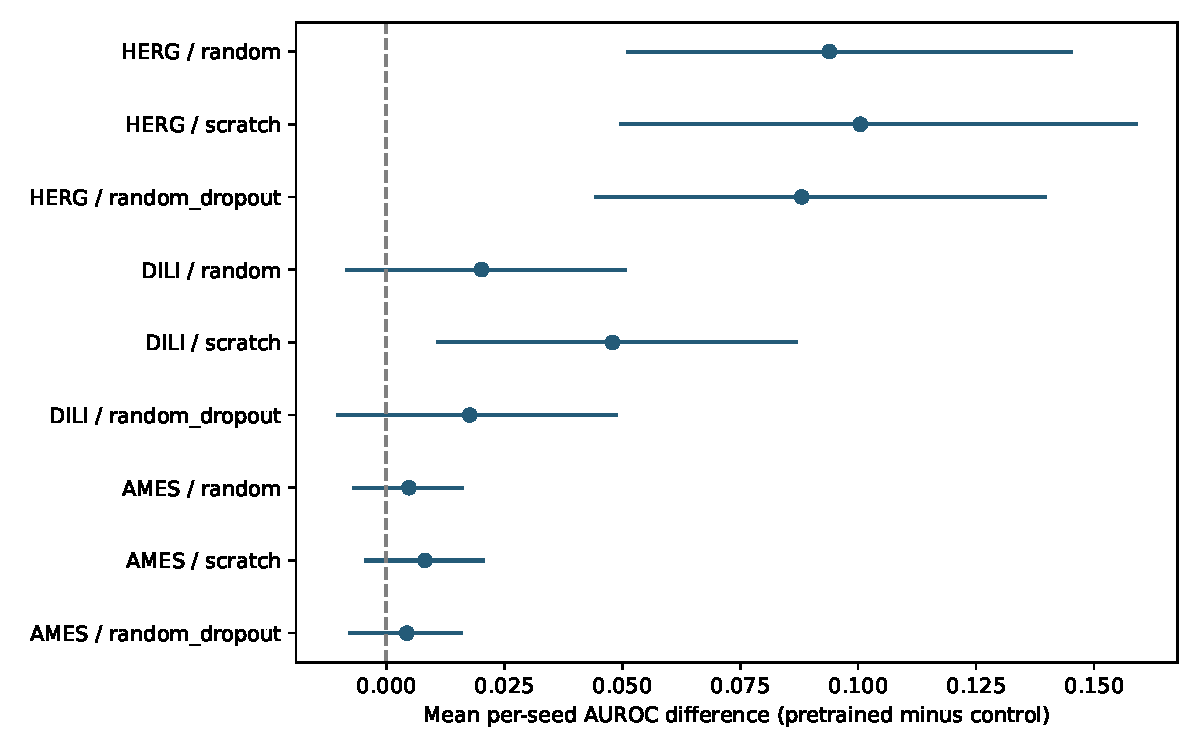
\includegraphics[width=.90\linewidth]{paired_initialization_effects.pdf}
\caption{Mean per-seed AUROC differences across five fixed partitions; random denotes Matched. Bars are 95\% percentile intervals from 5,000 coupled test-component and paired-seed resamples, conditional on the fitted models. These are not independent-study intervals or full retraining uncertainty. All nine contrasts are shown; multiplicity is reported in the text.}
\label{fig:effects}
\end{figure}

The corrected hERG advantage persists under the equal selection-only learning-rate grid: the selected-rate seed-mean AUROCs are \HergTunedPre{} and \HergTunedRandom{}. The aggregation factorial yields mean-pooling minus norm-pooling differences in the initialization gap of 0.0070--0.0238 across three seeds. These observations show that computation and optimization matter, but they do not identify a unique explanation for an old split's result. New partitions simultaneously change fitting populations, held-out composition, and component support. Their hERG mean initialization gaps range from \HergSplitMin{} to \HergSplitMax{}.

For training sizes 50, 100, 200, and 400, the low-data pretrained-minus-Matched mean differences are \LowDeltas{}. At size 50 the 95\% crossed-bootstrap interval is \LowFiftyCI{}, despite the positive mean. Sampling variation and the small common historical test set make a universal small-data advantage too strong. The design distinguishes a capacity contrast from a pretrained-weight contrast and does not reuse unsupported historical low-data $p$ values.

\begin{table}[t]
\centering
\caption{Secondary per-seed AUROC references. Panel A shares the five primary partitions; panel B has only one of them. Within each panel all listed fixed settings are retained. Differing tuning budgets and populations preclude a joint ranking.}\label{tab:secondary}
\small
\begin{tabular*}{.92\linewidth}{@{\extracolsep{\fill}}lrrr}
\toprule
Model & hERG & DILI & Ames\\
\midrule
\multicolumn{4}{l}{A: Classical references; five partitions (RF:25 fits; others:5)}\\
Random forest & 0.856 & 0.837 & 0.828\\
Histogram GB & 0.801 & 0.765 & 0.824\\
Logistic regression & 0.823 & 0.791 & 0.783\\
\midrule
\multicolumn{4}{l}{B: ChemBERTa; partition7301 only, three seeds at $10^{-4}$}\\
Pretrained & 0.872 & 0.787 & 0.807\\
Matched & 0.771 & 0.731 & 0.781\\
Scratch & 0.803 & 0.731 & 0.772\\
\bottomrule
\end{tabular*}
\end{table}


Table~\ref{tab:secondary} keeps classical references and the single-partition ChemBERTa experiment separate. Different partitions or tuning budgets cannot be interpreted as a common leaderboard. Historical code selected the highest-test-AUROC classical algorithm before inference; we retain that as a selection flaw and report all three fixed algorithms here. For ChemBERTa hERG, pretrained seed-mean AUROC is \HfHergSeed{}, whereas ensemble AUROC is \HfHergEnsemble{}. Matched's corresponding values are \HfRandomSeed{} and \HfRandomEnsemble{}: this concrete discrepancy shows why the two estimands must not be interchanged.

\subsection{Small probability changes can alter ranking}
Across the 672 BF16-trained neural models, raw-to-canonical maximum probability change is \MaxProbDrift{}. Test AUROC changes span \TestDriftMin{} to \TestDriftMax{}; these are evaluation-policy differences, distinct from repeated-BF16-forward instability. The maximum AUROC increase occurs in a hERG ChemBERTa Scratch run: raw AUROC 0.673148 versus canonical 0.818519. Raw predictions have only three distinct probabilities among 67 samples, versus 67 canonical values, despite a maximum probability difference of 0.002314. Independent scikit-learn computation verifies both AUROCs. We identify this as a descriptive extreme case, not a prespecified superiority test or a reason to choose the better-scoring policy.

The ten FP32-trained controls have identical raw and canonical predictions under the same deterministic evaluation. In hERG, their pretrained-minus-Matched AUROC gaps are \FpHergGaps{}, compared with \BfHergGaps{} for the paired BF16-trained models evaluated canonically. The two single-seed endpoints cannot establish general numerical stability. The evidence supports reporting an explicit execution policy and replay identity; it does not isolate a particular kernel or precision setting as the sole cause.

\subsection{Released-corpus matches do not identify causal exposure effects}
We reconstruct every nonblank record of the released corpus (Zenodo15733575 v1), identifying 944,296 lines, 944,168 raw unique InChIKeys, and 943,229 unique keys after symmetric standardization. The base checkpoint is the identified Zenodo15460715 v2 release; its full SHA256 and the corpus hash are preserved. The raw reconstructed set exactly equals the historical cache. Exact identity uses all InChIKey blocks; connectivity matching uses the first block. For historical test sets, raw exact/connectivity counts are 32/47 of 59 hERG structures, 47/48 of 51 DILI structures, and 522/597 of 732 Ames structures. Connectivity counts include exact matches.

These identify released-file matches, not complete checkpoint membership, ADMET-label exposure, or memorization. We freeze descriptor, fit-neighbor, and label-based propensity weights before reading new predictions, then compare the relative Brier benefit of pretraining across exact-matched/unmatched strata with unique test structures and common component resampling. Both identity rules are retained.

Adjusted hERG/Ames benefit-difference intervals include zero under both rules. DILI's unmatched effective sample size is 18.213, below the frozen threshold 20, so we do not estimate it. Unmeasured confounding, weight-fitting uncertainty, and actual training membership remain unresolved; no de-exposure intervention supports causal inflation claims.

\section{Calibration Isolation and Domain Shift}
For binary probabilities, the nonconformity score is $s(x,y)=1-p_y(x)$. With $n$ calibration scores and target error $\alpha$, we use the $k$th order statistic,
\begin{equation}
 k=\lceil(n+1)(1-\alpha)\rceil,\quad
 q=s_{(k)}\text{ if }k\leq n,\qquad q=+\infty\text{ otherwise},
\end{equation}
and predict the label set $C(x)=\{y:1-p_y(x)\leq q\}$. The implementation uses an inclusive boundary with tolerance $10^{-12}$. An infinite threshold yields the full label set rather than clipping the rank into the observed sample.

The main four-role analysis calibrates a locked five-seed ensemble on the independent calibration role. Coverage intervals resample calibration and test components separately, accounting for quantile and evaluation variability conditional on the fitted model. Platt and isotonic alternatives are fitted on selection only, before independent conformal calibration. We report every fixed alternative, not a test-selected best transform. Class-Mondrian and ten fit-only ECFP KMeans cells are also fixed without prediction outcomes; sparse cells retain the exact infinite-threshold rule. Cell support, class coverage, empty/full-set fractions, and pointwise intervals are recorded. Neither component resampling nor conditional partitioning restores exchangeability under scaffold shift.

\begin{table}[t]
\centering
\caption{Coverage summaries. Panel A ranges are descriptive extrema, not confidence intervals; per-split calibration/test-component intervals are in the evidence index. Panel B holds calibration size fixed. Its SD describes assignments over three fixed trajectories, not a standard error from 600 independent training runs. The two panels have different model/selection designs.}\label{tab:cp}
\small
\begin{tabular}{llrr}
\toprule
Endpoint / design & Target & Coverage & Variation\\
\midrule
\multicolumn{4}{l}{A: Independent calibration; five-partition mean [min,max]}\\
hERG & 0.9 & 0.952 & [0.910, 0.974]\\
hERG & 0.8 & 0.845 & [0.791, 0.909]\\
DILI & 0.9 & 0.926 & [0.908, 0.942]\\
DILI & 0.8 & 0.807 & [0.736, 0.855]\\
Ames & 0.9 & 0.899 & [0.883, 0.932]\\
Ames & 0.8 & 0.785 & [0.749, 0.822]\\
\midrule
\multicolumn{4}{l}{B: Ames reuse diagnostic; three trajectories $\times$200 assignments}\\
Calibration / evaluation & Target & Coverage & Across-assignment SD\\
Independent / pool & 0.9 & 0.903 & 0.019\\
Independent / scaffold & 0.9 & 0.873 & 0.017\\
Reused / pool & 0.9 & 0.897 & 0.022\\
Reused / scaffold & 0.9 & 0.866 & 0.018\\
\bottomrule
\end{tabular}
\end{table}


In the main partitions, independent-calibration coverage can be below or above nominal targets (Table~\ref{tab:cp}, panel A). These are descriptive split means; they are not simultaneous guarantees. A separate diagnostic addresses selection reuse with three fixed Ames training trajectories. For each trajectory, 20 saved candidates (epochs 5--100 in steps of 5) are evaluated canonically. Each of 200 randomized equal-size held-out-pool assignments creates a selection third, an independent calibration third, and a same-pool evaluation third. Selection AUROC chooses a candidate using only the selection third. The chosen predictor is calibrated either on that reused third or on the independent third, then evaluated on both the unused third and the fixed scaffold test set.

Equal calibration sizes prevent a sample-size explanation for the reuse contrast. At nominal 0.9, independent calibration has mean coverage \PoolIndependent{} within the held-out pool and \ShiftIndependent{} on the scaffold test set; reuse gives \PoolReused{} and \ShiftReused{}, respectively. These average the same 200 assignment indices across three fixed trajectories, not 600 independently trained models. The reuse comparison is randomized conditional on the trajectories; the domain comparison is observational and changes population composition. This distinction rules out a claim that reuse alone explains all observed undercoverage or that separating calibration guarantees coverage after structural shift.

Selective prediction uses full discrete AURC, averaging cumulative error over retained sizes $k=1,\ldots,n$, with the uniform within-tie-order expectation~\cite{geifman2017selective}. We retain four fixed scores: confidence, negative ensemble standard deviation, maximum fit similarity, and their equal-weight selection-standardized combination. All 240 point estimates and 360 paired compound/component contrast records are preserved. Historical AURC values and intervals are reproducible, but averaged only $k=20,\ldots,n$ with order-dependent tie breaking; they must not be mixed with the new definition.

\section{Limitations, Practical Implications, and Reproducibility}
Three inherited snapshots and one principal graph encoder do not provide a universal foundation-model ranking. CheMeleon's formal supporting information was inspected; its full formal main text was not recovered. Fixed classical settings, a single ChemBERTa partition, small test populations, overlapping source pools, and conditional bootstrap approximations limit generalization. Clinical/prospective selection outcomes were not measured.

Missing pIC50, measurement heterogeneity, and unresolved label aggregation prevent claiming independently approved ground truth. Neither strict-boundary filtering nor the Karim-derived sensitivity~\cite{karim2021cardiotox} establishes source independence. New external candidates remain quarantined and unscored; formal external admission and unresolved assay provenance are \textbf{BLOCKED}. No independent approval is asserted.

Practitioners should inspect computation before calling a control matched, enforce joint identity relations, separate seed-mean/ensemble estimands, replay fixed weights, and isolate score fitting, predictor selection, and calibration. Released-file matches require correspondingly limited language. These lessons follow without a claim that pretraining always helps or never helps.

The local package preserves protocols, hashes, row dispositions, checkpoints, probability versions, full metric/rate grids, bootstrap definitions, and claim-to-table mappings. Its 790 configurations comprise 643 graph models, 39 Transformers, 105 classical settings, and three trajectories; nine historical classical settings were reconstructed separately. Another 105 archival refits, 60 candidate states, and pool assignments are not independent training evidence. Execution used one RTX A2000 (6\,GB), PyTorch 2.6.0, Chemprop 2.3.1, and RDKit 2026.3.6. Ten contract tests pass; 1,752 original files, the main reference, and base checkpoint remain unchanged. Full training was not independently replayed bitwise.

The manuscript and local source bundle contain aggregates, without claiming public artifact access, approved member-level release, or anonymous deployment. New experiments do not retroactively validate uncertain historical $p$ values.

\section{Conclusion}
A computation-matched re-evaluation supports a conditional hERG initialization benefit while leaving DILI/Ames comparisons with the large random control uncertain. The audit additionally exposes historical pooling confounding, molecular identity dependencies, and ranking sensitivity to numerical execution. Released-corpus matching supports an observational identity statement, and independent calibration does not by itself establish structural-shift validity. Explicit estimands, preserved failure records, and fixed-weight replay make these conclusions inspectable without converting missing provenance or causal evidence into claims.

\paragraph{Writing disclosure.}
Generative AI assisted restructuring and drafting this research manuscript. This exceeds grammatical correction; the manuscript is not represented as compliant with PAKDD 2027's current AI-writing policy. Authors remain responsible for checking the evidence and obtaining applicable venue-policy clarification before submission.

\bibliographystyle{splncs04}
\bibliography{refs}
\end{document}
